\chapter{Analýza požadavků a návrh řešení}
\label{požadavky}
V~této kapitole je popsána analýza uživatele a jeho potřeb. Na základě uživatelem potřebných funkčností je zde proveden návrh databázové struktury, která v~sobě bude uchovávat informace potřebné pro vykonávání daných funkcí. Jako poslední obsahuje tato kapitola jednoduchý návrh grafického uživatelského prostředí na základě provedené analýzy uživatele.

\section{Cíl práce}

Cílem je dosáhnout funkční webové aplikace schopné pojmout jako vstup soubor formátu GEDCOM, tento soubor správně zpracovat, uložit potřebné informace a vytvořit záznamy o~chybějících informacích jednotlivých událostí. Tyto vytvořené záznamy je pak potřeba uživateli graficky zobrazit a navrhnout mu matriky, ve kterých by se informace mohly vyskytovat.

Hlavní myšlenkou je vytvořit aplikaci, která pomůže svým uživatelům s~dohledáním chybějících informací, tím že jim nabídne vhodné matriky, ve kterých by informace mohli najít. Tedy urychlit a usnadnit proces dohledávání informací.

\section{Uživatel a jeho potřeby} \label{uživatel_potřeby}

Uživatelem aplikace nemusí být pouze genealog, může se jednat o~jakoukoliv osobu provádějící genealogický výzkum. Aplikace je využívána k~ulehčení určování vhodných matrik pro vyhledávání chybějících informací v~již rozpracovaném GEDCOM souboru. Je tedy nutné aby uživatel byl schopen poskytnout tento soubor naplněný genealogickými daty. Aplikace nemá za úkol tyto soubory vytvářet, nýbrž pomáhat s~nalezením chybějících informací a musí tedy pracovat s~rozpracovanými soubory.

V~následujících kapitolách jsou vysvětleny funkce, které bude aplikace poskytovat svým uživatelům. Tyto funkce jsou také vyobrazeny v~diagramu případů užití (obrázek \ref{figure_usecase}).

\subsubsection{Práce se soubory}

Uživatel musí být schopen nahrát vstupní GEDCOM soubor do aplikace. U~nahrání souboru bude mít možnost jej pojmenovat a nastavit výpočetní parametry, které ovlivňují výpočty časových rozsahů. Aplikace mu umožní zobrazit si přehled nahraných souborů. U~těchto souborů bude moci editovat jméno, psát poznámky nebo je ze systému mazat. Soubory bude také schopen filtrovat nebo vyhledávat podle jména. Zároveň mu tyto soubory proklikem umožní dostat se na přehled záznamů vázaných k~tomuto souboru. V~rámci zpracování souboru bude uživatel povinen upřesnit území, které se v~souboru nedají jasně identifikovat. Při identifikaci mu bude aplikace nabízet území z~databáze.

\subsubsection{Záznamy}

Na přehledu zobrazující záznamy pro daný GEDCOM soubor si bude uživatel moci prohlížet vytvořené záznamy. Záznamy si bude moci filtrovat podle typu události, ke které jsou vázané. Se záznamem bude uživateli umožněno provádět různé operace. Mezi ty spadá možnost zobrazit si nabídnuté matriky, přes které se bude schopen dostat přímo na jejich detail v~digitálním archivu. Matriky bude také schopen odkliknout. Uživatel bude mít možnost záznam ignorovat nebo schválit. Schválení vybídne uživatele k~doplnění chybějících informací, při ignoraci aplikace přestane se záznamem pracovat. K~jednotlivým záznamům si bude uživatel také moci napsat poznámku.

\begin{figure}[H]
	\centering
	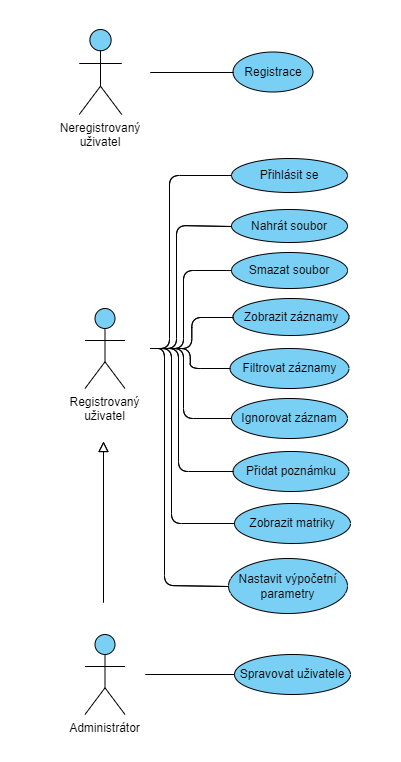
\includegraphics[height=152mm]{obrazky-figures/UseCase.png}
	\caption[Usecase]{Diagram případů užití}
	\label{figure_usecase}
\end{figure}

\section{Návrh databáze}

Návrh databáze je zde reprezentován pomocí diagramu vztahů mezi entitami\footnote{entita - objekt reálného světa zachycený v~datovém modelu} (ER\footnote{ER - Entity relationship}). V~rámci databáze MySQL jsou poté tyto jednotlivé entity a vztahy převedeny na tabulky na základě pravidel převodu. Entity nám zde představují jednotlivé objekty, se kterými pracujeme v~rámci aplikace. Jednotlivé entity a vztahy jsou pak popsány v~podkapitolách nacházejících se pod ER diagramem (obrázek \ref{figure_ER}).

\begin{figure}[H]
	\centering
	\includegraphics[width=150mm]{obrazky-figures/BCP\_ER.drawio.png}
	\caption[ER diagram]{Diagram vztahů mezi entitami}
	\label{figure_ER}
\end{figure}

\subsubsection{Uživatel}

Entita uživatel reprezentuje jednotlivé uživatele v~rámci aplikace. Slouží pro uchování základních informací o~uživateli jako jeho email, heslo a uživatelské jméno. Tato entita je důležitá, protože se k~ní váže entita GEDCOM souboru, kdy tento soubor musí vždy spadat pod nějakého uživatele.

\subsubsection{GEDCOM soubor}

Entita reprezentuje GEDCOM soubor v~rámci systému. Jejími atributy jsou jméno souboru a datum vytvoření. Tato entita je ve vztahu N:1 s~uživatelem, který ji vlastní. Dále je entita ve vztahu s~entitami Osoba a Rodina. Tato vazba reprezentuje osoby/rodiny nacházející se v~tomto souboru. Jsou ve vztahu 1:N.

\subsubsection{Osoba}

Jedná se o~entitu, která obsahuje záznamy o~konkrétních osobách nacházejících se v~nějakém GEDCOM souboru. Její atributy obsahují základní informace vytažené ze souboru, jako celé jméno, ID v~rámci souboru, pohlaví, ale hlavně informace týkající se sledovaných událostí. Tedy datum a místo narození/úmrtí. Osoba má vazbu vůči sama sobě, která určuje otce/matku dané osoby. Dále je osoba ve vztahu 1:N s~rodinou. Tato vazba znamená, že osoba v~rodině působí jako manžel/manželka, tedy i jako rodič pro ostatní členy rodiny. Osoba může být s~rodinou také ve vztahu N:1, kdy tato vazba znamená, že osoba působí v~rodině jako dítě.

\subsubsection{Rodina}

Rodina je v~aplikaci reprezentována pomocí stejnojmenné entity. Uchovává v~sobě informace o~události oddání. Je propojena několika vazbami s~entitou Osoba, které jsou popsány výše. Umožňuje reprezentovat vztahy mezi osobami v~rámci rodiny.

\subsubsection{Záznam}

V~případě, že u~události chybí nějaká informace je o~tom vytvořen záznam. Ten je v~aplikaci reprezentován entitou Záznam. Jeho atributem je typ popisující o~jakou událost se jedná. Dále pak umožňuje uživateli zapisovat k~sobě poznámky uložené do stejnojmenného atributu. Je ve vztahu s~entitami Osoba a Rodina, kdy pro osobu mohou existovat maximálně 2 záznamy a pro rodinu jeden. Dále je ve vztahu M:N s~entitou Matrika, kdy tento vztah vyjadřuje matriky nabídnuté k~danému záznamu.

\subsubsection{Matrika}

Tato entita slouží k~popsání jednotlivých matrik používaných v~aplikaci. Obsahuje mnoho atributů, hlavními jsou rozsahy od/do pro jednotlivé události, které nám říkají jaké události v~sobě matrika uchovává a mezi jakými roky. Dále pak obsahuje atributy určené k~odlišení matrik při zobrazení v~grafickém prostředí, jako původce a jeho typ. Atribut url pak umožňuje aplikaci přesměrovat uživatele na detail konkrétní matriky. Entita se nachází ve vztahu s~entitou Území, kdy tento vztah popisuje jaké území daná matrika pokrývá. Dále je pak ve vztahu se záznamem, jenž je popsán v~předchozí podkapitole.

\subsubsection{Území}

Jedná se o~entitu, jež představuje jednotlivé územní celky v~rámci České republiky. Obsahuje název celku, typ, o~který se jedná, a dále pak zeměpisnou šířku a délku popsanou pomocí souřadnic. Území je v~unárním vztahu samo se sebou, který říká, že nějaké území může být součástí jiného, většího území. Dále je pak ve vztahu s~matrikou, pod kterou spadá.

\section{Návrh uživatelského prostředí}
Jak bylo zmíněno v~podkapitole \ref{uživatel_potřeby} aplikace musí poskytovat uživateli nějaké funkcionality. Ty poskytuje prostřednictvím grafického rozhraní. V~této podkapitole budou zobrazeny jednoduché návrhy takového rozhraní pro jednotlivé funkcionality. V~rámci návrhu chceme zachovat minimalistický a jednoduchý vzhled, který uživatele dovede přímo ke chtěným operacím za použití co nejméně přechodů mezi stránkami.

\subsubsection{Práce se soubory}
Aplikace by měla obsahovat nějakou stránku s~přehledem souborů. V~naší aplikaci bude touto stránkou naše hlavní strana. Zde se bude nacházet jednoduchá tabulka obsahující nahrané soubory, které budou řazeny podle data nahrání. V~rámci této tabulky bude uživatel schopen provádět dříve zmíněné operace. Zároveň bude tuto tabulku používat k~přístupům na stránku, která bude zobrazovat jednotlivé záznamy vytvořené pro daný soubor. 
Na této stránce bude uživatel schopen také nahrát svůj soubor za pomocí tlačítka a vyskakovacího okna.

\begin{figure}[H]
	\centering
	\includegraphics[width=130mm]{obrazky-figures/návrh\_main\_menu.png}
	\caption[Návrh stránky souborů]{Stránka souborů - tabulka souborů}
	\label{figure_hlavní_stránka}
\end{figure}

\subsubsection{Záznamy}

Nejdůležitější stránkou aplikace bude ta, která zobrazí jednotlivé vytvořené záznamy souborů. Stránka by měla indikovat, který soubor právě zkoumáme nějakým nadpisem. Záznamy zde budou rozděleny podle jejich typu a možnost přecházet mezi typy bude uživateli dostupná bez nutnosti prokliku. Záznamy budou zobrazeny jinou formou nežli tabulkovou pro zpříjemnění práce s~aplikací. K~zobrazení záznamů budou tedy využity kartičky. Matriky navržené k~jednotlivým záznamům by měli být přidruženy ke kartičkám, aby opět nebylo nutné přecházet na jinou stránku.

\begin{figure}[H]
	\centering
	\includegraphics[width=130mm]{obrazky-figures/návrh\_karty.png}
	\caption[Návrh stránky záznamů]{Stránka záznamů - zobrazení kartiček}
	\label{figure_záznamy}
\end{figure}

\subsubsection{Poznámky}

Vytváření poznámek by mělo být uživateli přístupné u~jednotlivých objektů, kterých se budou týkat. Jejich vytváření by opět mělo proběhnout na stejné stránce. Využijeme k~tomu tedy zase vyskakovací okénko. Uživatel by měl mít možnost si někde zobrazit všechny poznámky pohromadě. K~tomu bude sloužit samostatná stránka tvořená tabulkou zobrazující jednotlivé poznámky tvořené pro konkrétní typy objektů. Návrh poznámkového okna je vyobrazen na obrázku \ref{figure_poznámka}

\begin{figure}[H]
	\centering
	\includegraphics[width=90mm]{obrazky-figures/návrh\_poznámka.png}
	\caption[Návrh okna poznámky]{Vyskakovací okno - editace poznámky}
	\label{figure_poznámka}
\end{figure}